\section{C vs C++}

\subsection{Differentiate between C and C++}
\begin{tabularx}{\textwidth}{|p{3.5cm}|X|X|}
    \hline \rowcolor{tableheader}
    \textbf{Aspect}                    & \textbf{C}                           & \textbf{C++} \\
    \hline \textbf{Paradigm}           & Procedural                           & Multi-paradigm (procedural, OOP, generic) \\
    \hline \textbf{Features}           & Simple, minimalistic                 & Object-oriented, templates, exceptions \\
    \hline \textbf{Standard Libraries} & Standard C Library                   & Standard Template Library (STL) \\
    \hline \textbf{Compatibility}      & More portable                        & Includes C features; additional features may not be universally supported \\
    \hline \textbf{Execution Speed}    & Often slightly faster                & Higher-level abstractions may incur overhead \\
    \hline \textbf{Memory Management}  & Manual (malloc, free)                & Manual and automatic (RAII, smart pointers) \\
    \hline \textbf{Usage}              & System programming, embedded systems & Larger-scale software, GUI applications \\
    \hline
\end{tabularx}

\begin{tcolorbox}[title=C]
\begin{verbatim}
#include <stdio.h>

int main() {
    printf("Hello, C!\n");
    return 0;
}
\end{verbatim}
\end{tcolorbox}

\begin{tcolorbox}[title=C++]
\begin{verbatim}
#include <iostream>

int main() {
    std::cout << "Hello, C++!" << std::endl;
    return 0;
}
\end{verbatim}
\end{tcolorbox}


\subsection{What is the difference between \texttt{cout} and \texttt{printf} in C++?}
\begin{tabularx}{\textwidth}{|p{3.5cm}|X|X|}
    \hline \rowcolor{tableheader}
    \textbf{Aspect}          & \texttt{cout}                                  & \texttt{printf}                               \\
    \hline
    \textbf{Usage}           & Part of C++ Standard Library (\texttt{<iostream>}) & Part of C Standard Library (\texttt{<stdio.h>}) \\
    \hline
    \textbf{Output}          & Formatted output to standard output            & Formatted output to standard output           \\
    \hline
    \textbf{Syntax}          & Uses \texttt{<<} insertion operator           & Uses format specifiers (\texttt{\%})          \\
    \hline
    \textbf{Type Safety}     & Type-safe; checks types at compile-time       & Format specifiers must match argument types  \\
    \hline
    \textbf{C++ Compatibility} & Native to C++, supports namespaces, exceptions & From C, compatible with C++ but lacks some C++ features \\
    \hline
    \textbf{Performance}     & Generally slower due to object-oriented nature & Generally faster for large-scale formatted output \\
    \hline
    \textbf{Buffer}          & It is fully buffered                           & It is line buffered \\
    \hline
    \textbf{Implementation}  & It is an object of \texttt{ostream} class      & It is a function \\
    \hline
\end{tabularx}

\subsection{What is the difference between \texttt{new} and \texttt{malloc()} in C++?}
\begin{tabularx}{\textwidth}{|p{2.5cm}|X|X|}
    \hline \rowcolor{tableheader}
    \textbf{Aspect}         & \texttt{new}                                          & \texttt{malloc()}                                    \\
    \hline
    \textbf{Language}       & C++                                                   & C                                                     \\
    \hline
    \textbf{Header File}    & \texttt{<new>} (automatically included in C++)       & \texttt{<stdlib.h>}                                   \\
    \hline
    \textbf{Return Type}    & Returns pointer to allocated memory of specific type & Returns \texttt{void*} (generic pointer)               \\
    \hline
    \textbf{Initialization}& Calls constructor for objects (if applicable)         & Memory allocated but no initialization                \\
    \hline
    \textbf{Type Safety}    & Type-safe; allocates memory for specific data type   & Not type-safe; requires casting for proper use         \\
    \hline
\end{tabularx}

\begin{tcolorbox}[title=new]
\begin{verbatim}
int* ptr = new int;
MyClass* obj = new MyClass();

delete ptr;
delete obj;
\end{verbatim}
\end{tcolorbox}

\begin{tcolorbox}[title=malloc]
\begin{verbatim}
int* ptr = (int*)malloc(sizeof(int)); // No equivalent for constructor invocation

free(ptr);
free(obj); // assuming obj is a pointer
\end{verbatim}
\end{tcolorbox}


\subsection{How do you link a C++ program to C functions?}
In C++, functions and variables are typically subject to name mangling—a process that encodes function signatures into unique names to support function overloading and type-safe linkage. However, when interfacing with C functions, which do not undergo name mangling, the \texttt{extern "C"} linkage specification is used to ensure compatibility and proper linking.

\begin{itemize}
    \item \textbf{Name Mangling:}
    \begin{itemize}
        \item C++ compilers encode function signatures into mangled names to handle function overloading and maintain type safety.
    \end{itemize}
    
    \item \textbf{C Functions:}
    \begin{itemize}
        \item C functions do not undergo name mangling and have straightforward function names.
    \end{itemize}
    
    \item \textbf{\texttt{extern "C"} Linkage Specification:}
    \begin{itemize}
        \item By using \texttt{extern "C"} around C function declarations in C++ code, you inform the compiler to disable name mangling for these functions. This allows the linker to correctly resolve and link function calls to their corresponding C function definitions.
    \end{itemize}
    
    \item \textbf{Compilation and Linking:}
    \begin{itemize}
        \item When compiling a C++ program that includes headers with \texttt{extern "C"} declarations, the compiler ensures that function names are not mangled.
        \item This enables the linker to correctly match calls from C++ code to the unmangled names of C functions defined elsewhere.
    \end{itemize}
\end{itemize}    

\begin{tcolorbox}[title=C Function to C++]
\begin{verbatim}
// C header file example.h
#ifdef __cplusplus
extern "C" {
#endif

void c_function(); // Declaration of C function

#ifdef __cplusplus
}
#endif
\end{verbatim}
\end{tcolorbox}


\subsection{Differences between struct in C and C++.}
\begin{tabularx}{\textwidth}{|p{2.5cm}|X|X|}
    \hline \rowcolor{tableheader}
    \textbf{Aspect}                 & \textbf{C}                                      & \textbf{C++}                                             \\
    \hline
    \textbf{Default Access Specifier} & No default; members default to \texttt{public} & Default access specifier is \texttt{public}                 \\
    \hline
    \textbf{Keyword Usage}           & Requires \texttt{struct} keyword               & Does not require \texttt{struct} keyword                   \\
    \hline
    \textbf{Member Functions}        & Cannot have member functions                  & Can have member functions (methods)                         \\
    \hline
    \textbf{Inheritance}             & Does not support inheritance                 & Supports single and multiple inheritance                    \\
    \hline
    \textbf{Constructor}             & No constructors                               & Can have constructors and destructors                       \\
    \hline
    \textbf{Access Control}          & No access control (all members public by default) & Supports access specifiers (\texttt{public}, \texttt{private}, \texttt{protected}) \\
    \hline
\end{tabularx}
\begin{tcolorbox}[arc=5pt, boxrule=2pt, title=Notes]
\textbf{Keyword Usage:} In C, you must use the \texttt{struct} keyword when declaring a struct variable (\texttt{struct Point p;}). In C++, the \texttt{struct} keyword is optional (\texttt{Point p;}).
\end{tcolorbox}

\subsection{What does extern "C" int func(int *, Foo) accomplish?}
In C++, the \texttt{extern "C"} declaration is used to specify that the function \texttt{func} should use C-style linkage rather than C++ linkage. This affects how the function's name is represented (or mangled) by the compiler, which is crucial for interoperability between C++ code and code written in other languages like C.

\begin{itemize}
    \item \textbf{Name Mangling:}
    \begin{itemize}
        \item C++ compilers often "mangle" function names, meaning they encode additional information about a function's parameters and return type into the function's name. This allows for function overloading and is used to implement features like namespaces.
    \end{itemize}
    
    \item \textbf{C-style Linkage:}
    \begin{itemize}
        \item When you declare a function with \texttt{extern "C"}, you're telling the compiler to use C-style linkage for that function. This linkage does not perform name mangling, resulting in a plain function name without any additional encoding.
    \end{itemize}
    
    \item \textbf{Purpose:}
    \begin{itemize}
        \item The \texttt{extern "C"} declaration is typically used when you need to interface with code that has been compiled using a C compiler. Since C compilers do not perform name mangling, using \texttt{extern "C"} ensures that the function's name remains unchanged and can be correctly referenced from C code.
    \end{itemize}
\end{itemize}

\begin{tcolorbox}[title=Extern C]
\begin{verbatim}
// C++ code
extern "C" {
    int func(int* ptr, Foo obj);  // Declares func with C-style linkage
}
\end{verbatim}
\end{tcolorbox}


\subsection{}



% Dummy section to be used with charts
\subsection{Simple Flowchart}

\tikzstyle{startstop} = [rectangle, rounded corners, minimum width=3cm, minimum height=1cm,text centered, draw=black, fill=red!30]
\tikzstyle{process} = [rectangle, minimum width=3cm, minimum height=1cm, text centered, draw=black, fill=orange!30]
\tikzstyle{decision} = [diamond, minimum width=3cm, minimum height=1cm, text centered, draw=black, fill=green!30]
\tikzstyle{arrow} = [thick,->,>=stealth]
\begin{center}
\begin{tikzpicture}[node distance=2cm]
    \node (start) [startstop] {Start};
    \node (process1) [process, below of=start] {Process 1};
    \node (decision1) [decision, below of=process1, yshift=-1cm] {Decision 1};
    \node (process2a) [process, below of=decision1, yshift=-1cm] {Process 2a};
    \node (process2b) [process, right of=decision1, xshift=3cm] {Process 2b};
    \node (stop) [startstop, below of=process2a] {Stop};

    \draw [arrow] (start) -- (process1);
    \draw [arrow] (process1) -- (decision1);
    \draw [arrow] (decision1) -- node[anchor=east] {Yes} (process2a);
    \draw [arrow] (decision1) -- node[anchor=south] {No} (process2b);
    \draw [arrow] (process2a) -- (stop);
    \draw [arrow] (process2b.east) -- ++(1,0) |- (process1.east);
\end{tikzpicture}
\end{center}


\subsection{Decision Tree}
\begin{center}
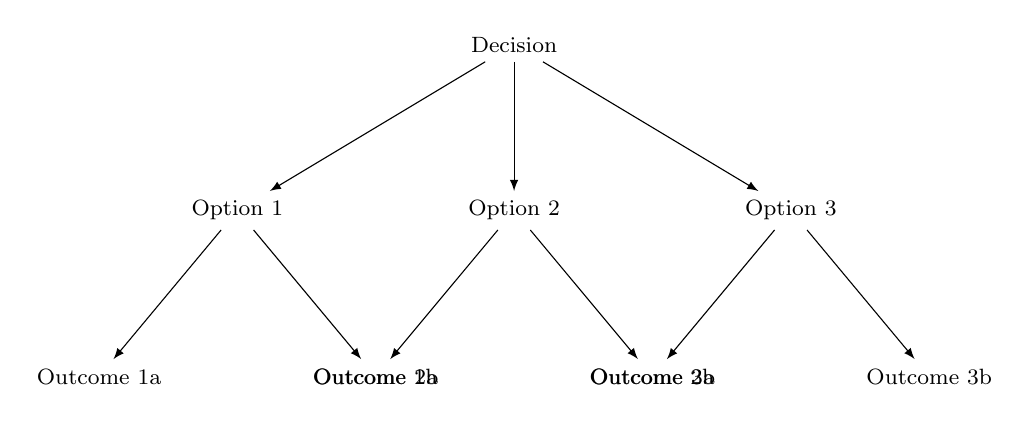
\begin{tikzpicture}[
    edge from parent/.style={draw, -latex},
    sibling distance=10em, level distance=6em,
    every node/.style={font=\footnotesize}]
    
    \node {Decision}
        child { node {Option 1}
            child { node {Outcome 1a} }
            child { node {Outcome 1b} }
        }
        child { node {Option 2}
            child { node {Outcome 2a} }
            child { node {Outcome 2b} }
        }
        child { node {Option 3}
            child { node {Outcome 3a} }
            child { node {Outcome 3b} }
        };
\end{tikzpicture}
\end{center}

\subsection{Data Flow Diagram}
\tikzstyle{process} = [rectangle, minimum width=3cm, minimum height=1cm, text centered, draw=black, fill=orange!30]
\tikzstyle{data} = [trapezium, trapezium left angle=70, trapezium right angle=110, minimum width=2cm, minimum height=1cm, text centered, draw=black, fill=yellow!30]
\tikzstyle{arrow} = [thick,->,>=stealth]

\begin{tikzpicture}[node distance=1.5cm]
    \node (input) [data] {Input Data};
    \node (process1) [process, right of=input, xshift=3cm] {Process 1};
    \node (data) [data, below of=process1, yshift=-1cm] {Stored Data};
    \node (process2) [process, right of=process1, xshift=3cm] {Process 2};
    \node (output) [data, right of=process2, xshift=3cm] {Output Data};

    \draw [arrow] (input) -- (process1);
    \draw [arrow] (process1) -- (data);
    \draw [arrow] (data) -- (process2);
    \draw [arrow] (process2) -- (output);
    \draw [arrow] (data.north) -- ++(0,1) -| (process2.south);
\end{tikzpicture}


\subsection{Class Diagram}
\begin{center}
\begin{tikzpicture}[
    class/.style={
        rectangle,
        draw=black,
        fill=blue!20,
        text centered,
        minimum width=3cm,
        minimum height=2cm
    },
    relation/.style={
        -{stealth[open]},
        thick
    },
    aggregation/.style={
        -{diamond[open]},
        thick
    },
    composition/.style={
        -{diamond[fill=black]},
        thick
    },
    generalization/.style={
        -{stealth[open]},
        thick
    }
]

\node[class] (classA) {
    \begin{tabular}{c}
    \textbf{Class A} \\
    \hline
    +attribute1 \\
    +attribute2
    \end{tabular}
};
\node[class] (classB) [below left=of classA] {
    \begin{tabular}{c}
    \textbf{Class B} \\
    \hline
    +attribute3 \\
    +attribute4
    \end{tabular}
};
\node[class] (classC) [below right=of classA] {
    \begin{tabular}{c}
    \textbf{Class C} \\
    \hline
    +attribute5 \\
    +attribute6
    \end{tabular}
};

\draw[relation] (classA) -- (classB) node[midway, fill=white] {1..*};
\draw[aggregation] (classA) -- (classC) node[midway, fill=white] {1};
\draw[composition] (classB) -- (classC) node[midway, fill=white] {0..1};

\end{tikzpicture}
\end{center}